To create a TikZ LaTeX diagram that visually represents the trees \( T_i \) for \( 1 \leq i \leq 5 \) and their corresponding sets of red vertices \( S_i \), while highlighting the pair \( u, v \) such that \( d_T(u, v) = i \) where condition \( i \) fails, we can follow these steps:

1. **Define the Trees**: Create five different trees with increasing distances between specific pairs of vertices.
2. **Highlight the Pair**: Mark the vertices \( u \) and \( v \) at the specified distance in each tree.
3. **Color Red Vertices**: Identify and color the vertices that form the set \( S_i \).

Here is a sample TikZ code to achieve this:

```latex
\documentclass{article}
\usepackage{tikz}

\begin{document}

\begin{figure}[h]
    \centering
    \begin{tabular}{c c c c c}
        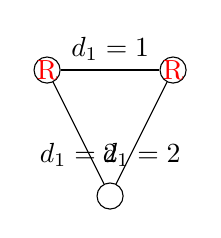
\begin{tikzpicture}[scale=0.8]
            \node[draw, circle] (A) at (0,0) {};
            \node[draw, circle] (B) at (2,0) {};
            \node[draw, circle] (C) at (1,-2) {};
            \draw (A) -- (B);
            \draw (A) -- (C);
            \draw (B) -- (C);
            \node[red] at (A) {R};
            \node[red] at (B) {R};
            \node at (C) {};
            \path (A) -- node[midway, above] {$d_1 = 1$} (B);
            \path (A) -- node[midway, below] {$d_1 = 2$} (C);
            \path (B) -- node[midway, below] {$d_1 = 2$} (C);
        \end{tikzpicture}
        &
        \begin{tikzpicture}[scale=0.8]
            \node[draw, circle] (A) at (0,0) {};
            \node[draw, circle] (B) at (2,0) {};
            \node[draw, circle] (C) at (4,0) {};
            \node[draw, circle] (D) at (2,-2